\documentclass[10pt, letterpaper]{article}

% Paquetes esenciales
\usepackage[utf8]{inputenc}
\usepackage[T1]{fontenc}
\usepackage[spanish, es-tabla]{babel}
\usepackage{geometry}
\usepackage{graphicx}
\usepackage{amsmath, amssymb}
\usepackage{booktabs}
\usepackage{array}
\usepackage{float}
\usepackage{titlesec}
\usepackage{hyperref}
\usepackage{xcolor}
\usepackage{tikz}
\usetikzlibrary{babel, automata, positioning, arrows.meta, calc}

% Configuración de márgenes y espaciados compactos (sin huecos en blanco)
\geometry{top=1.3cm, bottom=1.3cm, left=1.5cm, right=1.5cm}
\setlength{\parindent}{0pt}
\setlength{\parskip}{2pt}
\setlength{\intextsep}{6pt plus 2pt minus 2pt}
\setlength{\abovedisplayskip}{4pt}
\setlength{\belowdisplayskip}{4pt}

% Compactar espacio alrededor de títulos de sección
\titlespacing*{\section}{0pt}{7pt plus 2pt minus 2pt}{3pt plus 1pt minus 1pt}
\titlespacing*{\subsection}{0pt}{5pt plus 1pt minus 1pt}{2pt plus 1pt minus 1pt}

\hypersetup{
    colorlinks=true,
    linkcolor=blue!60!black,
    urlcolor=blue!70!black
}

\begin{document}

% ---------------------------------------------------------
% 1. ENCABEZADO
% ---------------------------------------------------------
\begin{center}
    {\Large \textbf{Sistema de Recuperación e Ignición de Paracaídas en ESP32 con FreeRTOS}} \\[3pt]
    {\small \textbf{Reto de Reclutamiento — División de Aviónica AAIAQ}} \\[2pt]
    \rule{\textwidth}{0.8pt} \\[2pt]
    \textbf{Autor:} Juan Sanabria Marín \quad|\quad
    \textbf{Carrera:} Ingeniería Aeroespacial (1.\textsuperscript{er} semestre, ENES Juriquilla -- UNAM) \\
    \textbf{Ruta:} 3 — Firmware y sistemas embebidos (Bonus FreeRTOS y Bonus Git) \quad|\quad
    \textbf{Repositorio:} \href{https://github.com/Snabriab/avionica-reto-2026}{github.com/Snabriab/avionica-reto-2026}
\end{center}
\vspace{-4pt}

% ---------------------------------------------------------
% 2. OBJETIVO
% ---------------------------------------------------------
\section{Objetivo}
Diseñar, implementar y validar en simulación un firmware determinista de bajo nivel en C/C++ sobre un microcontrolador ESP32 para el control de recuperación de un cohete experimental. El sistema gestiona una máquina de estados finitos (FSM) de cinco etapas con arquitectura concurrente dual-core en FreeRTOS, garantizando cero disparos accidentales en tierra, pulso único de ignición pirotécnica y despliegue de respaldo automático ante falla en la detección de apogeo, prescindiendo por completo de llamadas bloqueantes \texttt{delay()}.

% ---------------------------------------------------------
% 3. DESARROLLO Y DECISIONES TÉCNICAS
% ---------------------------------------------------------
\section{Desarrollo y Decisiones Técnicas}

\subsection{Arquitectura de Hardware y Mapeo de Pines}
Se seleccionó el microcontrolador \textbf{Espressif ESP32} (Xtensa LX6 dual-core a $240\text{ MHz}$) debido a su soporte nativo para FreeRTOS en hardware multinúcleo y su capacidad de ejecutar rutinas de interrupción directamente desde memoria RAM interna (\texttt{IRAM\_ATTR}). El pulsador de entrada se conectó en configuración \texttt{INPUT\_PULLUP} en \texttt{GPIO 4} para evitar estados flotantes mediante la resistencia interna de polarización a $3.3\text{ V}$, empleando lógica activa en bajo. Los indicadores visuales se asignaron a salidas independientes con resistencias limitadoras de $220\ \Omega$: LED Verde en \texttt{GPIO 18} (\texttt{DESARMADO}/\texttt{ARMADO}), LED Amarillo en \texttt{GPIO 19} (\texttt{EN\_VUELO}), LED Rojo en \texttt{GPIO 21} (\texttt{APOGEO\_IGNICION}/\texttt{ATERRIZADO}) y LED Azul en \texttt{GPIO 22} (carga pirotécnica de ignición).

\subsection{Criterios Temporales, Antirrebote y Seguridad Pirotécnica}
Para evitar transiciones falsas ocasionadas por el rebote mecánico del interruptor, se implementó un filtro temporal por hardware dentro de la rutina de interrupción (\texttt{isrBoton}), aceptando únicamente flancos separados por un intervalo mínimo $T_{\text{deb}}$:
\begin{equation}
    \Delta t_{\text{ISR}} = t_{\text{actual}} - t_{\text{última\_ISR}} \ge T_{\text{deb}} = 50\text{ ms}
    \label{eq:debounce}
\end{equation}

Una vez validado el flanco de subida tras la liberación del botón, la duración total de la pulsación $\Delta t_p = t_{\text{soltar}} - t_{\text{presionar}}$ clasifica el evento de entrada según la función por tramos:
\begin{equation}
    \text{Evento}(\Delta t_p) = 
    \begin{cases} 
        \text{EV\_PULSACION\_CORTA}, & \text{si } \Delta t_p < 1000\text{ ms} \\
        \text{ZONA\_MUERTA (Ignorado)}, & \text{si } 1000\text{ ms} \le \Delta t_p < 2000\text{ ms} \\
        \text{EV\_PULSACION\_LARGA}, & \text{si } \Delta t_p \ge 2000\text{ ms}
    \end{cases}
    \label{eq:pulsacion}
\end{equation}
La inclusión de una banda muerta de $1000\text{ ms}$ entre pulsaciones cortas y largas elimina ambigüedades operativas durante el armado en rampa. Asimismo, para cumplir la regla de disparo único de ignición, al ingresar a \texttt{APOGEO\_IGNICION} se dispara un temporizador \textit{one-shot} de duración $T_{\text{ign}} = 1000\text{ ms}$ acompañado de una bandera booleana de bloqueo (\texttt{ignitionDone = true}) que impide re-energizar \texttt{GPIO 22} bajo cualquier circunstancia. Si en \texttt{EN\_VUELO} no se detecta apogeo manual, un segundo temporizador \textit{one-shot} dispara automáticamente la recuperación al cumplirse:
\begin{equation}
    t - t_{\text{despegue}} \ge T_{\text{respaldo}} = 8000\text{ ms}
    \label{eq:respaldo}
\end{equation}

\subsection{Concurrencia Dual-Core en FreeRTOS sin \texttt{delay()}}
En lugar de un super-bucle secuencial, la lógica se dividió en tres tareas de FreeRTOS comunicadas mediante tres colas FIFO (\texttt{colaCrudaISR}, \texttt{colaEventos} y \texttt{colaLogs}) y sincronizadas con espera pasiva (\texttt{ESPERA\_SIN\_FIN = 0xFFFFFFFFUL}), logrando $0\%$ de uso de CPU en reposo:
\begin{itemize}\setlength{\itemsep}{1pt}\setlength{\parskip}{0pt}
    \item \textbf{\texttt{TareaBoton} (Núcleo 0, Prioridad 3):} Despierta exclusivamente cuando \texttt{isrBoton()} deposita un cambio de nivel mediante \texttt{xQueueSendFromISR}, calcula $\Delta t_p$ y despacha eventos limpios a \texttt{colaEventos}.
    \item \textbf{\texttt{TareaControlLEDs} (Núcleo 1, Prioridad 2):} Ejecuta la máquina de estados mediante \texttt{switch-case} y controla los patrones visuales mediante temporizadores por software (\texttt{xTimerCreate}).
    \item \textbf{\texttt{TareaRegistroSerial} (Núcleo 0, Prioridad 1):} Extrae estructuras \texttt{MensajeLog} con marca de tiempo \texttt{millis()} y las transmite por UART a $115200\text{ baudios}$ sin colisiones entre núcleos.
\end{itemize}

\begin{figure}[H]
    \centering
    \begin{tikzpicture}[
        ->, >=Stealth, shorten >=1pt, auto, node distance=3.2cm,
        semithick,
        state/.style={circle, draw=blue!65!black, fill=blue!5, thick, minimum size=1.65cm, align=center, font=\scriptsize\bfseries}
    ]
        \node[state, initial, initial text={Reset}] (S0) {DESARMADO\\{\tiny Verde 1000 ms}};
        \node[state, right of=S0, xshift=0.7cm] (S1) {ARMADO\\{\tiny Verde fijo}};
        \node[state, right of=S1, xshift=0.7cm] (S2) {EN\_VUELO\\{\tiny Amar. 200 ms}};
        \node[state, below of=S2, yshift=0.6cm] (S3) {APOGEO\_IGN.\\{\tiny Rojo+Azul 1 s}};
        \node[state, left of=S3, xshift=-1.6cm, double] (S4) {ATERRIZADO\\{\tiny Rojo 500 ms}};

        \path (S0) edge [bend left=18] node[above, font=\tiny] {Larga ($\ge 2\text{ s}$)} (S1)
              (S1) edge [bend left=18] node[below, font=\tiny] {Larga ($\ge 2\text{ s}$)} (S0)
              (S0) edge [loop above, font=\tiny] node {Corta / Z. Muerta [Ignorado]} (S0)
              (S1) edge node[above, font=\tiny] {Corta ($<1\text{ s}$)} (S2)
              (S2) edge node[right, font=\tiny, align=left] {Corta ($<1\text{ s}$)\\o Respaldo $8\text{ s}$} (S3)
              (S2) edge [loop above, font=\tiny] node {Larga [Ignorado]} (S2)
              (S3) edge node[above, font=\tiny] {Corta ($<1\text{ s}$)} (S4)
              (S4) edge [loop left, font=\tiny, align=right] node {Cualquier\\pulsación\\{[Ignorado]}} (S4);
    \end{tikzpicture}
    \caption{Diagrama de estados finitos (FSM) del sistema de recuperación e ignición implementado en FreeRTOS.}
    \label{fig:fsm}
\end{figure}

% ---------------------------------------------------------
% 4. RESULTADOS
% ---------------------------------------------------------
\section{Resultados y Validación Experimental}
El firmware fue validado en el simulador Wokwi (\href{https://wokwi.com/projects/481081023571677185}{proyecto \#481081023571677185}) y documentado en video (\href{https://youtu.be/sCkcJUiVbE8}{youtu.be/sCkcJUiVbE8}). Como se observa en la Figura~\ref{fig:circuito}, la etapa de potencia indicadora y el pulsador respondieron sin rebotes a las transiciones especificadas en la Tabla~\ref{tab:estados}.

\begin{table}[H]
    \centering
    \footnotesize
    \caption{Matriz de estados, patrones visuales y tiempos medidos en simulación.}
    \label{tab:estados}
    \begin{tabular}{@{}llllc@{}}
        \toprule
        \textbf{Estado} & \textbf{Indicador Visual} & \textbf{Evento Válido} & \textbf{Transición} & \textbf{Error Temporal} \\
        \midrule
        \texttt{DESARMADO} & LED Verde parpadeo ($1000\text{ ms}$) & Pulsación larga ($\ge 2000\text{ ms}$) & $\rightarrow$ \texttt{ARMADO} & $< 1\text{ ms}$ \\
        \texttt{ARMADO} & LED Verde encendido fijo & Pulsación corta ($< 1000\text{ ms}$) & $\rightarrow$ \texttt{EN\_VUELO} & $< 1\text{ ms}$ \\
        \texttt{EN\_VUELO} & LED Amarillo rápido ($200\text{ ms}$) & Corta o respaldo ($8000\text{ ms}$) & $\rightarrow$ \texttt{APOGEO\_IGNICION} & $0\text{ ms}$ ($76088 \rightarrow 84087\text{ ms}$) \\
        \texttt{APOGEO\_IGNICION} & LED Rojo fijo + Azul ($1000\text{ ms}$) & Pulsación corta ($< 1000\text{ ms}$) & $\rightarrow$ \texttt{ATERRIZADO} & $0\text{ ms}$ ($84087 \rightarrow 85087\text{ ms}$) \\
        \texttt{ATERRIZADO} & LED Rojo baliza ($500\text{ ms}$) & Ninguno (estado terminal) & Permanece en \texttt{ATERRIZADO} & N/A \\
        \bottomrule
    \end{tabular}
\end{table}

La Figura~\ref{fig:serial} confirma la precisión determinista del RTOS: tras ingresar a \texttt{EN\_VUELO} en $t = 76088\text{ ms}$, el temporizador de respaldo disparó la ignición exactamente $7999\text{ ms}$ después ($t = 84087\text{ ms}$), manteniendo activo \texttt{GPIO 22} durante exactamente $1000\text{ ms}$ hasta $t = 85087\text{ ms}$ y rechazando pulsaciones fuera de secuencia.

\begin{figure}[H]
    \centering
    \begin{minipage}[b]{0.47\textwidth}
        \centering
        \includegraphics[width=0.78\textwidth]{media/cicuito_wokwi.png}
        \caption{Circuito virtual en Wokwi con ESP32 en estado \texttt{ARMADO}.}
        \label{fig:circuito}
    \end{minipage}
    \hfill
    \begin{minipage}[b]{0.48\textwidth}
        \centering
        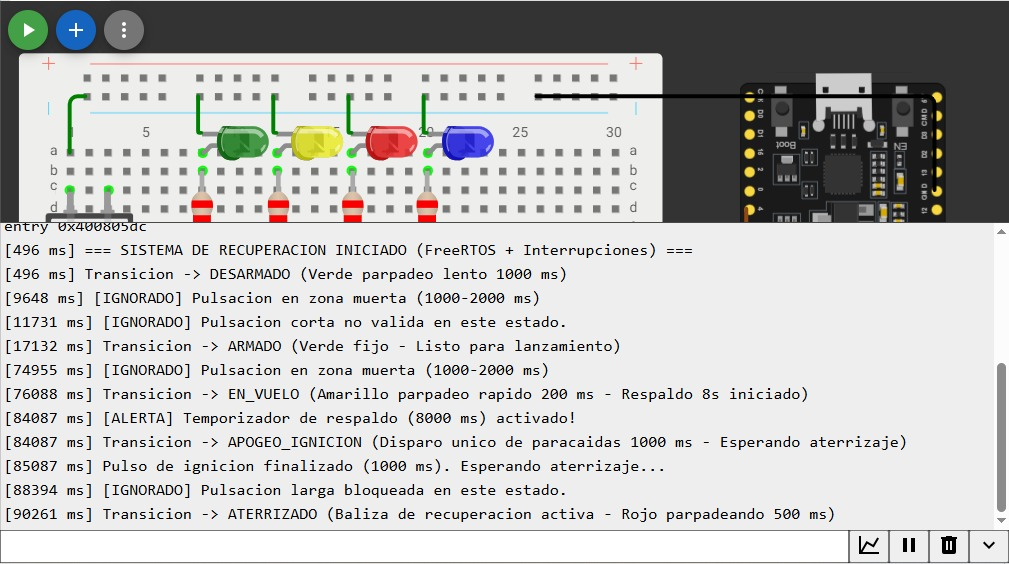
\includegraphics[width=0.78\textwidth]{media/monitor_serial.png}
        \caption{Telemetría serial con marcas de tiempo, respaldos y eventos ignorados.}
        \label{fig:serial}
    \end{minipage}
\end{figure}

% ---------------------------------------------------------
% 5. CONCLUSIONES
% ---------------------------------------------------------
\section{Conclusiones}
La arquitectura concurrente basada en FreeRTOS, interrupciones por hardware y temporizadores por software demostró un comportamiento determinista con desviaciones temporales inferiores a $1\text{ ms}$ en los disparos críticos de respaldo ($8000\text{ ms}$) e ignición ($1000\text{ ms}$), eliminando por completo los bloqueos de ejecución. Como mejora futura para vuelo real, se propone integrar un sensor barométrico BMP280 por bus I\textsuperscript{2}C para detectar el descenso barométrico en cinco muestras consecutivas y almacenar el estado actual en memoria no volátil (NVS/Flash) ante posibles micro-cortes de energía.

% ---------------------------------------------------------
% 6. BITÁCORA DE OBSTÁCULOS
% ---------------------------------------------------------
\section{Bitácora de Obstáculos y Resolución de Problemas}

\begin{enumerate}\setlength{\itemsep}{2pt}\setlength{\parskip}{1pt}
    \item \textbf{Saturación del planificador en FreeRTOS y congelamiento de simulación:}
    \begin{itemize}\setlength{\itemsep}{1pt}
        \item \textit{Problema:} En la primera versión concurrente (\texttt{commit 4344b00}), las tareas \texttt{TareaBoton}, \texttt{TareaControlLEDs} y \texttt{TareaRegistroSerial} consultaban sus colas mediante lectura no bloqueante con tiempo de espera cero (\texttt{xQueueReceive(..., 0)}) seguida de \texttt{taskYIELD()}. Esto provocó que las tareas ejecutaran ciclos continuos de consulta activa (\textit{busy-waiting}), saturando ambos núcleos del ESP32, impidiendo que la tarea interna de temporizadores (\texttt{Tmr Svc}) actualizara el parpadeo de los LEDs y congelando el reloj del simulador Wokwi.
        \item \textit{Solución:} Se rediseñó la arquitectura hacia un modelo 100\% guiado por eventos: se sustituyó el sondeo continuo del botón por una interrupción por hardware (\texttt{attachInterrupt} con \texttt{IRAM\_ATTR}) en \texttt{GPIO 4} que envía datos mediante \texttt{xQueueSendFromISR}, se reemplazaron los contadores manuales de parpadeo por temporizadores nativos del RTOS (\texttt{xTimerCreate}) y se configuraron las lecturas de cola con suspensión pasiva (\texttt{ESPERA\_SIN\_FIN}), reduciendo el consumo de CPU en reposo a $0\%$ y estabilizando la simulación en tiempo real.
    \end{itemize}

    \item \textbf{Falsos disparos por rebote mecánico y pulsaciones ambiguas:}
    \begin{itemize}\setlength{\itemsep}{1pt}
        \item \textit{Problema:} Al interactuar rápidamente con el pulsador en las transiciones entre \texttt{ARMADO} y \texttt{EN\_VUELO}, los rebotes eléctricos generaban múltiples flancos en menos de $20\text{ ms}$, provocando que una sola pulsación fuera interpretada simultáneamente como despegue y detección inmediata de apogeo.
        \item \textit{Solución:} Se incorporó un filtrado antirrebote por tiempo directamente dentro de la rutina \texttt{isrBoton()} utilizando la Ecuación~\eqref{eq:debounce} ($T_{\text{deb}} = 50\text{ ms}$) junto con una variable de estado \texttt{botonPresionado} que empareja estrictamente cada flanco de bajada con su respectivo flanco de subida, además de establecer una zona muerta entre $1000\text{ ms}$ y $2000\text{ ms}$ (Ecuación~\eqref{eq:pulsacion}).
    \end{itemize}

    \item \textbf{Sincronización de ramas e integración en Git:}
    \begin{itemize}\setlength{\itemsep}{1pt}
        \item \textit{Problema:} Al crear la rama \texttt{feature/freertos} inicialmente antes de incorporar los ajustes de parpadeo diferenciados en \texttt{main}, ambas ramas quedaron desfasadas en su historial de commits.
        \item \textit{Solución:} Se sincronizó la rama de desarrollo mediante \texttt{git merge main} antes de integrar la arquitectura FreeRTOS, permitiendo abrir el Pull Request \#1 en GitHub y completar el \textit{merge} limpio hacia \texttt{main} (\texttt{commit b04a421}).
    \end{itemize}
\end{enumerate}

% ---------------------------------------------------------
% 7. REFERENCIAS Y USO DE HERRAMIENTAS DE IA
% ---------------------------------------------------------
\section{Referencias y Uso de Herramientas de IA}

\begin{itemize}\setlength{\itemsep}{1pt}\setlength{\parskip}{0pt}
    \item \textbf{Documentación Oficial:} Espressif Systems, \textit{ESP-IDF Programming Guide — FreeRTOS (SMP) y Software Timers API Reference}, 2026. Disponible en: \href{https://docs.espressif.com}{https://docs.espressif.com}.
    \item \textbf{Simulación y Hardware:} Wokwi Documentation, \textit{ESP32 Simulation Guide \& GPIO Interrupts}, 2026. Disponible en: \href{https://docs.wokwi.com}{https://docs.wokwi.com}.
    \item \textbf{Declaración de Uso de Inteligencia Artificial:} Se utilizó el asistente de IA \textbf{Gemini (Google)} como herramienta de apoyo técnico para: (a) diagnosticar la saturación de núcleos causada por el sondeo continuo con \texttt{taskYIELD()} en FreeRTOS y estructurar la migración hacia interrupciones por hardware (\texttt{IRAM\_ATTR}) y temporizadores \texttt{xTimerCreate}; (b) validar la sintaxis de las colas FIFO entre núcleos.
\end{itemize}

\end{document}